\documentclass[10pt]{report}
\usepackage{epsf}
\usepackage{amsmath}
\usepackage{amssymb}
\usepackage{float}
\usepackage{palatino}
\usepackage[pdftex]{graphics}
\usepackage{fancyhdr}
\usepackage[pdftex]{graphicx}
\usepackage{hyperref}
\parindent 0in
\parskip 1ex
\oddsidemargin  0in
\evensidemargin 0in
\textheight 8.5in
\textwidth 6.5in
\topmargin -0.25in

\pagestyle{fancy}
\fancyhf{}
\fancyhead[L]{\bf BME354L - Palmeri - Spring 2013}
\fancyhead[R]{{\bf Arduino Project}}
%\fancyfoot[L]{LICENSE: CC BC-NC-SA 3.0 ({\tt http://creativecommons.org/licenses/by-nc-sa/3.0/})}
\fancyfoot[C]{\thepage}

\title{Microcontrollers and Embedded Systems}
\author{Will Scheideler}
\begin{document}

\section*{Microcontrollers and Embedded Systems}

\subsection*{Introduction}
Hi and welcome to BME 354! This class integrates many concepts from Electrical Engineering and Biomedical Engineering, from circuit design to signal processing. This semester, we are putting a greater emphasis on microcontrollers and embedded programming, in light of how ubiquitous they are. Today, almost every electronic device, from toaster ovens to heart rate monitors, uses some sort of microcontroller. For the first time, BME 354 will introduce a final project involving the Arduino Uno hardware platform. Throughout the semester, we will post a series of small tutorials to get you comfortable working with the Arduino Uno so the project will be a very natural transition.
\par
I realize those of you taking this class come from different backgrounds-some may be ECE’s with a strong background in programming, others may be BME’s with little interest in this area. For the ECE’s, some of the content in these tutorial may be very easy for you, but I still encourage you to play around with the Arduino and maybe you’ll discover something cool. For the BME’s, I hope this series of tutorials generates some interest in embedded systems, at the very least bestow some general knowledge about microcontrollers that is very important in the biomedical engineering industry today.

\subsection*{What is a microcontroller?}

A microcontroller is essentially a small computer. It is a small integrated circuit (as opposed to a circuit with discrete components, an IC has all its circuit components printed onto a single chip) that is able to run computer code, take inputs, and control outputs. As a result of being printed, IC’s are often really very small (you’ve already worked with IC’s in the form of the AD620 and LF353 op-amps). In contrast to the microprocessors used in say your laptop, microcontrollers are designed for embedded applications (this means they usually perform a very specific task, are lower power and lower cost). 
\par
They are often used in devices that don’t necessarily need all the functionality of your laptop’s Intel Core i7; for example, a remote control only needs to be able to detect the user’s button presses, transmit some sort of signal to your television, and do all this with as long a battery life as possible. Some devices, such as a toaster oven, were originally built without microcontrollers at all. However, as you will see, microcontrollers have many benefits: they are cheap, are often more reliable than mechanical components, and can be programmed for greater functionality. Many medical devices can be categorized as embedded systems, with a specific function to perform. With the advent of many portable and implanted medical devices, specialized system-on-a-chip designs are becoming increasingly relevant. The Arduino Uno platform uses an ATMega328P microcontroller. The Uno is pictured in Figure 1 and that long, black component is the microcontroller.

\begin{figure}[H]
\centering
   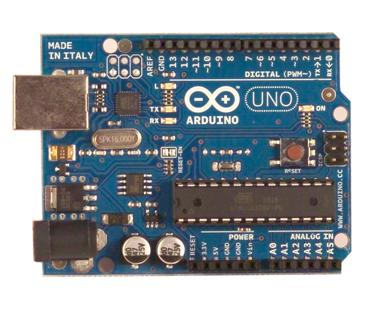
\includegraphics[width=0.5\textwidth]{arduino.jpg}
    \caption{A view of the Arduino board.}
\end{figure}

\subsection*{Microcontroller Breakdown}

So, how does a microcontroller work? How do we characterize its performance and capabilities? Here are some terms that you should be familiar with when working with the Arduino. These terms will help you understand the data sheets and other sources that reference these characteristics.

 \begin{itemize}
\item \textbf{Operating Voltage} - This is supply voltage (Vdd) of the development board; the USB cable or power jack will supply this voltage to the board. The Arduino Uno’s operating voltage is 5V; another common operating voltage is 3.3V (useful for devices powered by 3.7V LiI cells, i.e. your cellphone). The Arduino is also built with a Vin pin that allows for an alternative supply voltage.
  
\item \textbf{Frequency} – Also called the clock. This is a signal that oscillates between +/- Vdd that controls how many instructions the microcontroller will execute every second. On the Arduino Uno, the clock is 16 MHz and is dictated by a ceramic resonator (a piezoelectric component that oscillates when you pass a voltage through it). For comparison, your laptop is probably clocked at around 2 GHz.

\item \textbf{Memory}
\begin{itemize}

\item Flash: This is kind of like the hard drive on your computer. It’s non-volatile memory, meaning that when you turn the power off, the data stored in this memory will not be erased. This is where the program and your variables are stored.

\item EEPROM: This is also nonvolatile memory. It is used to store long term information. It can only be accessed using read() and write().

\item SRAM: This is like the ram in your computer, so it is volatile memory, meaning that it will be cleared if your turn the power off. It is used by the Arduino to perform calculations and operations on your variables.

\end{itemize}
\end{itemize}

\subsection*{Arduino I/O}

I/O stands for input/output. Input and output refer to the signals that are transmitted to and from an embedded systems. Inputs to the microcontroller may originate as signals of nearly any kind (i.e. pressure, temperature, height, force, magnetic field, conductivity, etc). The good news is that transducers exist to convert these signals to voltages. A microcontroller then reads the voltage at an input pin and processes these voltage signals before giving feedback to the system. Feedback originates as voltage at an output pin of the microcontroller. Transducers convert this signal back into other forms of energy. Figure 2, below, illustrates this process.

\begin{figure}[H]
\centering
   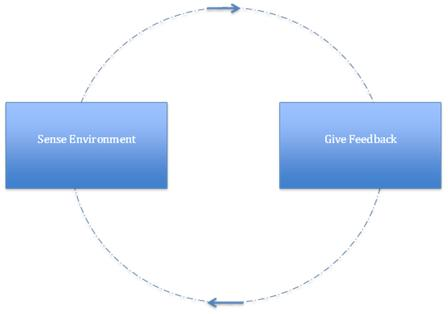
\includegraphics[width=0.4\textwidth]{feedback.jpg}
    \caption{General scheme of an embedded system.}
\end{figure}

\begin{itemize}

\item \textbf{Digital IO} – The Arduino has many pins to interface with hardware outside of the board. There are 14 digital pins that can act as inputs or outputs. The default state of any pin on the Arduino is input. (Can you guess why this is the case?). In Input mode, digital pins have a high input impedance (approximately $100 M \Omega$). A digital input reads a voltage signal and converts that voltage signal to a single bit of information ( 1 or 0 ).  As an output, the digital pins will convert a 1 / 0 to Vdd / GND. The digital pin can source or sink up to 40 mA of current. This is enough for most applications (Powering a sensor or an LED), but not enough power for something like a motor.

\item \textbf{Analog IO} - On the other side of the board, there are 6 analog pins ($A0 – A5$) that can be used to sense analog voltage levels (or may be used as general purpose digital pins). Each analog pin is attached to a 10-bit ADC that has a dynamic range of GND to Vdd. An external voltage level (Vref) that is applied to the Vref pin can also be used as an upper reference voltage to enhance the sensitivity of ADC measurements. Analog input pins have similar properties to digital input pins (high input impedance) that make them favorable for measuring low-level signals from a variety of sensors.

\item \textbf{PWM} – The Arduino is equipped with 6 pins that can output PWM signals (marked with a $\sim$ on the board). \textbf{Pulse width modulation} refers to a method of creating a square wave with a variable duty cycle. Figure  below shows square waves with a variable duty cycle. As shown, the duty cycle is the percentage of time that the output is HIGH. Pulse width modulation is a method that is often used to control the delivery of power to a load (i.e. Switched Converters, bridge circuits for driving a motor, etc). When the frequency is fast enough, we can adjust say, the brightness of an LED, imperceptible to the user that it is actually blinking on and off very fast. As you learn to design embedded systems, you will discover the usefulness of dedicated PWM outputs.

\end{itemize}

\begin{figure}[H]
\centering
   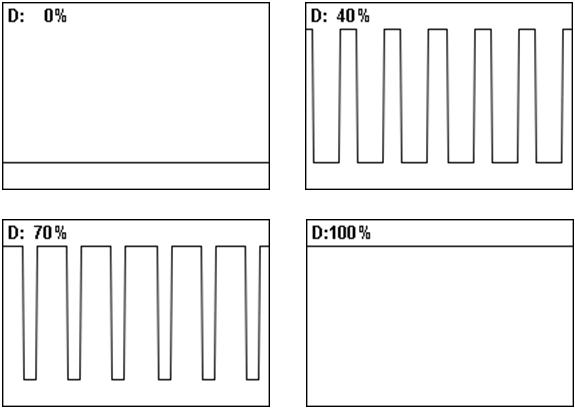
\includegraphics[width=0.9\textwidth]{dutyCycle.jpg}
    \caption{PWM signals with variable duty cycles..}
\end{figure}

\subsection*{Programming the Arduino}

\par 
So now that you are familiar with some of the hardware features of the Arduino, it’s time to take a look at the software side and how the Arduino actually does what you program it to do. So this is a super brief glimpse at computer engineering and I know I may lose some of you so let me know if you’re confused about anything. Nothing here will be on your test, it’s all just for your own understanding.
\par
The first concept we should introduce is that the microcontroller, just like any other computer processor, is a \textbf{digital system}. This means that it can ONLY represent discrete values. For the most part, they can only take values of 0 or 1, represent by low and high voltages, respectively. The digital system operates by reading long sequences of 0’s and 1’s.
\par 
\textbf{High level programming} – This is the type of programming you are probably most familiar with. This includes common programming languages like Java, Python, C, C++, Javascript, and so on. These languages were created so humans could easily write computer programs, a logical arrangement of instructions. However, this is not what a computer’s processor actually sees; remember, the processor is a digital system, so it can only understand 0’s and 1’s. To do so, there are two levels of translation that need to happen.
\par
The first is the compiler. The \textbf{compiler} converts a high level language such as C into a low level language, otherwise known as an assembly language, such as MIPS or x86. Assembly languages don’t have complicated functions or variable types and instead only use instructions that the processor can easily understand. The set of instructions that the processor understands is called the instruction set architecture. However, this is still not what the processor sees.
\par
One thing of note though – you can actually program the Arduino using assembly. Using assembly might be useful if you want to know EXACTLY what the processor is doing, literally every single instruction. This allows you to have precise control over how optimized your program is for that specific task.
\par
The second level of translation is the assembler. The assembler converts low-level assembly language into binary code, or machine language. Each instruction has it’s own unique combination of binary code that the assembler translates to.
\par
So now we have a big list of binary codes. Each one is the same length. In a 32-bit machine, these codes are 32 bits long. In a 64-bit machine, these codes are 64 bits long. The computer will simply execute each one in order. This is where the clock comes in. Every time the clock “ticks,” the processor knows to execute one instruction. Obviously, the faster the clock cycle, the more instructions it can perform per second. If the clock is too fast though, then the processor might not have finished the previous instruction, and you will get messed up data. Additionally, a faster clock usually requires more power, which may very well be a consideration for medical devices.
\par
I won’t dive too deeply into what kinds of things assembly languages can and can’t do, or how processors execute each instruction – that is for ECE 250, computer architecture, if any of you are interested. Just know that processors execute machine language, which is assembled from assembly language, which is compiled from high level languages.

\subsection*{Why Arduino?}
There are a several advantages to using Arduino.

\begin{itemize}
\item
Arduino is a great board to learn embedded programming on. It is based on the C++ programming language, but hides a lot of the technical stuff from the user. As such, it is very easy to get up and running. The whole vision of the Arduino line of development boards was that it could allow anyone to easily pick up and build cool electronics. That said, while it is a good introduction to design and a quick way to build cool stuff, it won’t teach you a lot of the technical details that you have to really muck around with in other microcontrollers such as PIC or AVR. So just know its limitations.
\item
It is very simple to interface with. Whereas the PIC would require you to download MPLAB, which is quite a heavy Integrated Developing Environment (IDE), Arduino’s text editor like IDE is very lightweight and simple. Additionally, there is no need for an additional programmer; Arduino simply interfaces with USB. Again, this goes with the whole “easy to pick up” theme.
\item
There is a lot of hardware support for the Arduino. Many companies sell shields that increase the hardware capabilities of the Arduino so the user doesn’t have to build hardware for common tasks. For example, there are LCD shields for displaying text and numbers, there are Ethernet shields and Wifi shields for connecting to the Internet, and there are audio shields to play high quality music.
\item
Lastly, and most importantly, there is a huge amount of open source software available online. The massive user base contributes a lot of code for common functions to entire projects. People have made electronic instruments, light-up clothing and costumes, automate household appliances, and even medical devices and much, much more. If you are interested, take a look online and see what people have made, some of these projects are really cool.

\end{itemize}

\end{document}